\chapter{Software Libraries \& Lab Infrastructure}\label{chp:apx:infrastructure}
\dropcap{I}n this Appendix, we present multiple software libraries and packages that were developed as part of the Ph.D and are all openly hosted within the \texttt{tud-phi} organization on GitHub~\footnote{\url{https://github.com/tud-phi}}. Furthermore, we report on essential components of the lab infrastructure that the Ph.D. candidate significantly contributed to.
% While these are all technical instead of scientific contributions, their development took significant effort, they were essential for the scientific results presented in this thesis, and we believe that sharing that sharing these technical will be valuable for the community and furthering the research in this domain.
Although these contributions are technical rather than scientific, their development required considerable effort and was crucial to achieving the scientific results presented in this thesis. We believe that sharing these technical resources will be valuable for the community and help advance research in this domain.

% For example, we envision the description of ROS2 package for Optitrack \gls{MCS}, the Festo pressure regulator including pneumatic circuitry schematic and ROS2 drivers to be helpful for soft robotic practitioners in establishing their own experimental setup.
% Furthermore, the JAX implementation of soft robotic dynamic models takes a step towards modernizing the soft robot algorithmic software stack and enable researchers to in the future leverage techniques such as auto differentation, \gls{JIT}-compilation, and deployment on \glspl{GPU} with soft robotic models, which is also crucial when integrating those into \gls{ML} approaches.
For instance, we anticipate that the ROS2 package for Optitrack \gls{MCS}, along with the Festo pressure regulator documentation—including its pneumatic circuitry schematic and ROS2 drivers—will be valuable for soft robotics practitioners setting up their own experimental systems. Additionally, our JAX implementation of soft robotic dynamic models marks a step toward modernizing the algorithmic software stack, enabling researchers to leverage techniques such as automatic differentiation, \gls{JIT}-compilation, and \gls{GPU} deployment, which are essential for integrating these models into \gls{ML} approaches. 
% Finally, we the fullfledged \gls{HSA} software ecosystem will allow the community to quickly bootstrap their \gls{HSA} robot (control) research and inspire the development of similar ROS2 packages for other soft robots.
Finally, our fully-fledged \gls{HSA} software ecosystem will enable the community to rapidly bootstrap their \gls{HSA} robot control research and inspire the creation of similar ROS2 packages for other soft robots.

\section{Motion Capture System}\label{sec:apx:infrastructure:motion_capture_system}
% Our experiments with soft robots often require accurate information about the state of the robot.
% Examples include closed-loop control based on accurate state information, such as done in Chapter~\ref{chp:hsacontrol}, or as a ground truth for quantitatively evaluating proprioceptive shape sensing approaches, as needed in Chapters~\ref{chp:srslam} \& \ref{chp:promasens}.
% As common in both research and industry, we decided to use a \gls{MCS} system manufactured by Optitrack consisting of eight cameras with \gls{IR} illumination. Our trials need to be reproducible, and the effort required for setting up the experiments should be minimal. As \gls{MCS} systems require precise calibrations, which can be rather time-consuming to achieve and need to be repeated every time the pose of any camera is changed, we built a cubical cage of side length \SI{750}{mm} with standard aluminum t-beams. The cameras can be very flexibly mounted to the beams using clamps. This prevents us from having re-calibrating frequently as the poses of the cameras stay constant relative to each other.
Our soft robot experiments demand precise state information. For example, tasks like closed-loop control (as demonstrated in Chapter~\ref{chp:hsacontrol}) and the quantitative evaluation of proprioceptive shape sensing approaches (as outlined in Chapters~\ref{chp:srslam} and \ref{chp:promasens}) rely on accurate soft robot backbone shape information. In line with common practice in both research and industry, we use an Optitrack \gls{MCS} system equipped with eight \gls{IR}-illuminated cameras (Optitrack Prime X13). To ensure that our trials are reproducible while minimizing setup effort, we built a cubical cage with a \SI{750}{mm} side length using standard aluminum T-beams. The cameras are flexibly mounted to the beams with clamps, which keeps their relative positions fixed and eliminates the need for frequent, time-consuming recalibrations whenever a camera’s pose might change.

% To enable closed-loop control based on the \gls{MCS} measurements, we developed a ROS2 package building on the NatNet SDK which is available on GitHub~\footnote{\url{https://github.com/tud-phi/ros2-mocap_optitrack}} for streaming the poses of the tracked rigid bodies from the Windows workstation running the Optitrack Motive software and transforming the poses from the MoCap world frame into a soft robot base coordinate system, that has its origin at the soft robot's base and with the z-direction pointing along the backbone direction.
To enable closed-loop control using the \gls{MCS} measurements, we implemented a ROS2 package built on the NatNet SDK. This package, available on GitHub\footnote{\url{https://github.com/tud-phi/ros2-mocap_optitrack}}, streams the poses of tracked rigid bodies from a Windows workstation running the Optitrack Motive software and publishes them as ROS messages. Subsequently, the package transforms the poses from the MoCap world frame to a soft robot base coordinate system, with the origin at the robot’s base and the z-axis aligned with the backbone direction.

\begin{figure}[ht]
     \centering
     \includegraphics[width=0.8\textwidth]{appendix-infrastructure/figures/graphic_experimental_setup.drawio_v1.drawio_compressed.pdf}
     \caption{
     % Experimental setup with a pneumatic soft robot segment: A soft robotic segment is mounted to a cage with attached motion capture cameras. The segment is pneumatically actuated by a pressure regulator (Fest Motion Terminal). A workstation communicates with both the motion capture cameras and the pressure regulator via Ethernet.
     Experimental Setup with a Pneumatic Soft Robot Segment: A soft robotic segment is attached to the top of a cage equipped with motion capture cameras. Pneumatic actuation is achieved using a pressure regulator (Festo VTEM Motion Terminal), while a workstation manages communication via Ethernet with both the motion capture system and the pressure regulator.
     }
     \label{fig:apx:infrastructure:experimental_setup}
\end{figure}

\section{Pneumatic Pressure Regulator}
% As described previously, our soft robotic arm design is pneumatically actuated by regulating the air pressure in the segment chambers. In literature, one can find two main methods for pneumatic actuation: 
% \begin{enumerate}
%     \item \textbf{Fluidic Drive Cylinders:} In this case, the air chambers of the soft robot are connected to a set of fluidic drive cylinders~\citep{marchese2014design, taheri2014force}. By actuating the position of the pistons, the volume of the closed system can be adjusted, and thus, the pressure is changed under the ideal gas assumption inverse proportionally~\citep{stolzle2021piston}. 
%     \item \textbf{Valves:} Alternatively, the chambers are connected to pneumatic valves which regulate, on the one hand, the airflow from a high-pressure source into the chamber and, on the other hand, the air exchange with the environment at atmospheric pressure to release pressure~\citep{falkenhahn2016dynamic}.
% \end{enumerate}
In this thesis, we consider at various times (e.g., Chapters~\ref{chp:srslam}, \ref{chp:background}, \ref{chp:promasens}) pneumatically-actuated robots. Two primary methods exist for implementing such actuation. The first involves fluidic drive cylinders, where the robot’s air chambers are connected to an array of cylinders~\citep{marchese2014design, taheri2014force}. In this setup, moving the pistons adjusts the volume of the closed system, causing the pressure to change inversely according to the ideal gas law~\citep{stolzle2021piston} (see Chapter~\ref{chp:backstepping}). Alternatively, pneumatic valves can be used to manage airflow: they control the entry of air from a high-pressure source into the chamber and facilitate pressure release by allowing air to escape to the atmosphere~\citep{falkenhahn2016dynamic}.

% We decided to go with the second option and procured the \emph{Motion Terminal VTEM}\footnote{{\small \url{https://www.festo.com/de/en/p/motion-terminal-id_VTEM/}}} from Festo, which can be configured to regulate the airflow into 16 independent chambers.
% While we use its pressure regulation function primarily, it also supports flow control and many other control tasks. 
% A rather complex pneumatic circuitry is needed to connect the motion terminal to the air supply unit, which we document in Fig.~\ref{fig:apx:infrastructure:pressure_regulator_tubing_circuitry_scheme}.
% We communicate pressure set-points to the pressure regulator via Modbus/\gls{TCP} through a \gls{LAN}. The pre-configured, low-level PID controller of the pressure regulator adjusts the valve positions accordingly to reach the desired pressure set point. The currently measured pressures at the valves can also be accessed through Modbus/\gls{TCP} and used, for example, for system identification purposes.
% For the required Modbus/\gls{TCP} communicated, we have developed drivers in both C++ and MATLAB based on the VTEM protocol~\footnote{\url{https://www.festo.com/net/SupportPortal/Files/684271/VTEM_PLC_QuickReference_V1-4.pdf}}.
% The drivers are together with a ROS2 package available on GitHub~\footnote{\url{https://github.com/tud-phi/ros2-vtem_control/tree/main?tab=readme-ov-file}} and allow both publishings of pressure commands for each of the valves and subscription to the current pressure readings of each valve.
We opted for the valve-based approach and selected Festo’s \emph{Motion Terminal VTEM}\footnote{{\small \url{https://www.festo.com/de/en/p/motion-terminal-id_VTEM/}}}, which can regulate airflow into 16 independent chambers. Although pressure regulation is our primary focus, the VTEM also supports flow control and additional tasks. To connect the motion terminal with the air supply unit, we developed a sophisticated pneumatic circuitry (see Fig.~\ref{fig:apx:infrastructure:pressure_regulator_tubing_circuitry_scheme}). Pressure set-points are transmitted via Modbus/\gls{TCP} over a \gls{LAN}, and the regulator’s built-in low-level PID controller adjusts the valve positions to achieve these targets. Simultaneously, current pressure readings from the valves are made available for purposes such as system identification. For this communication, we developed drivers in both C++ and MATLAB based on the VTEM protocol\footnote{\url{https://www.festo.com/net/SupportPortal/Files/684271/VTEM_PLC_QuickReference_V1-4.pdf}}, which are distributed together with a ROS2 package on GitHub\footnote{\url{https://github.com/tud-phi/ros2-vtem_control}}. These tools allow users to both publish pressure commands and subscribe to the valve pressure data.

\begin{figure}[ht]
     \centering
     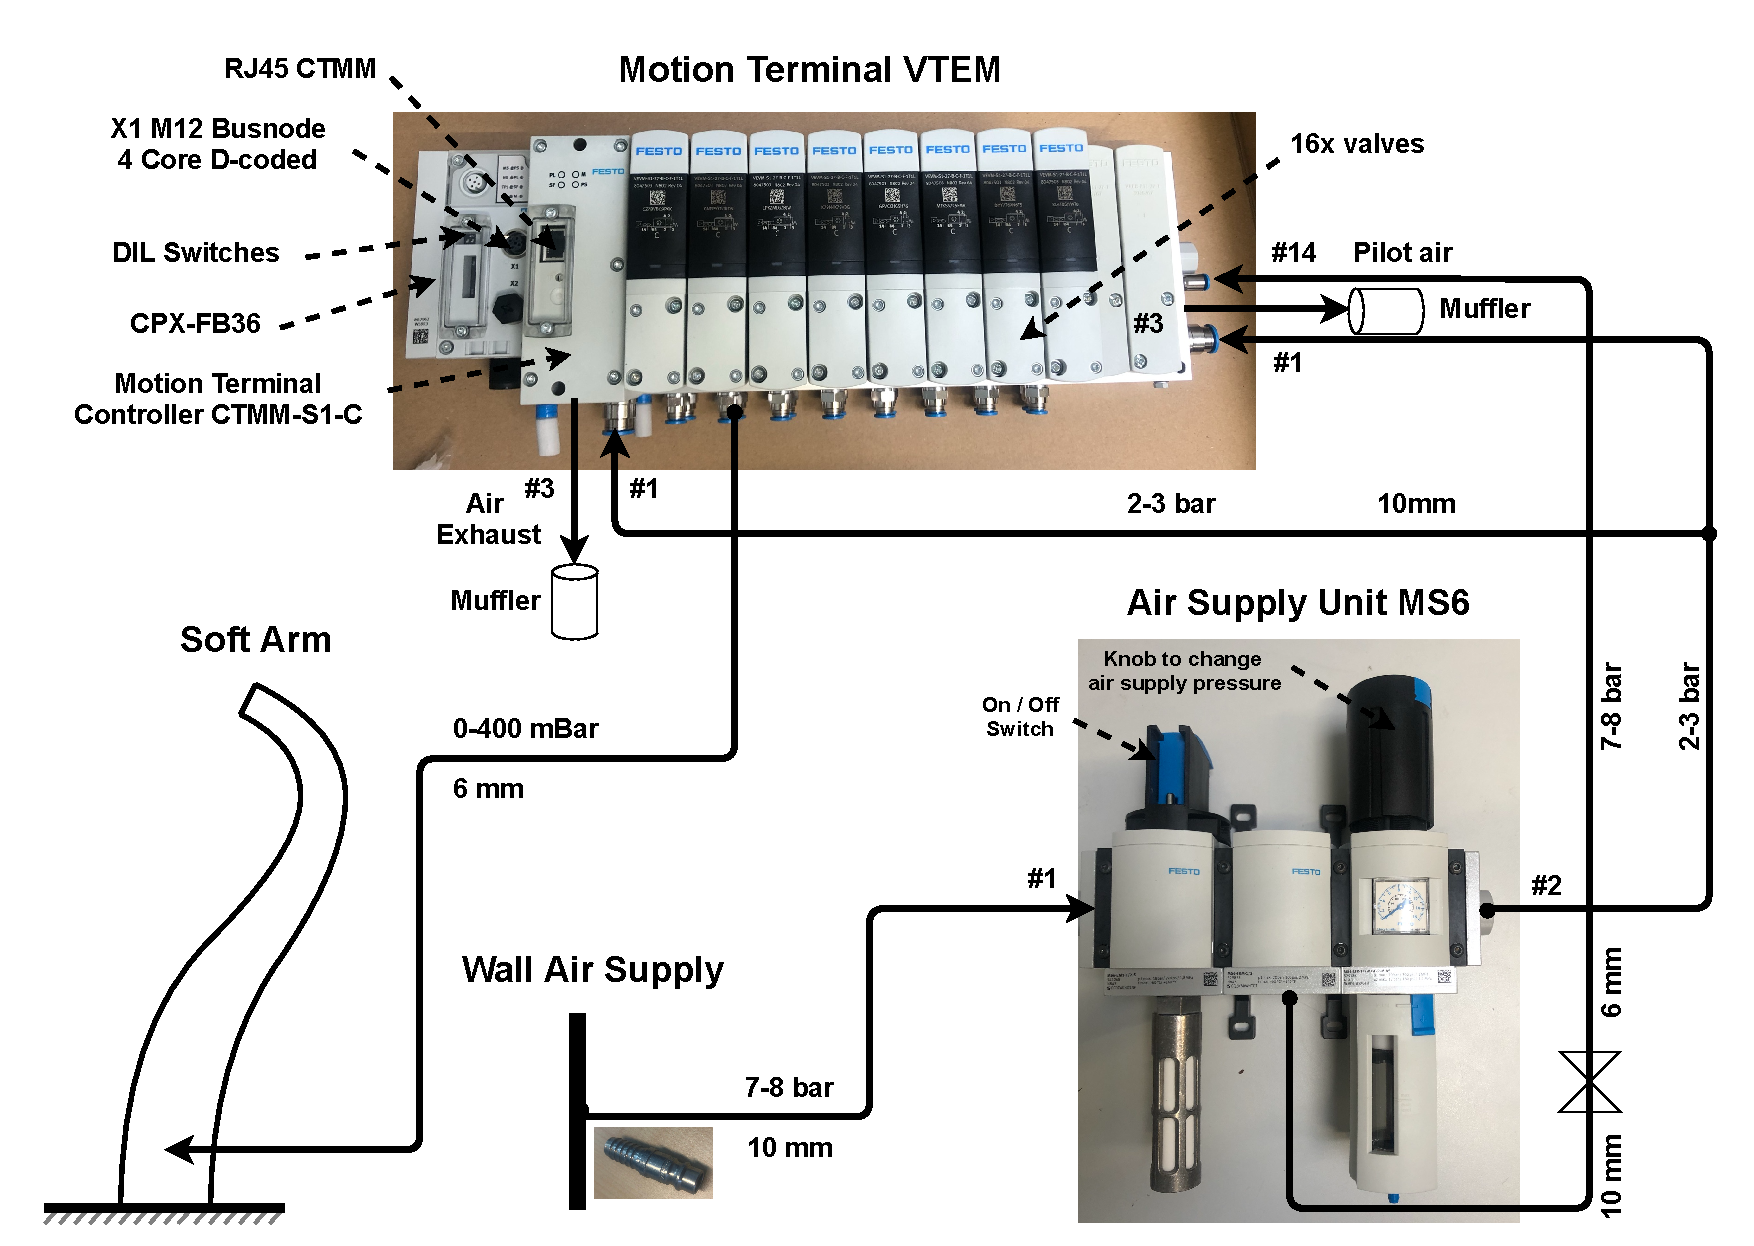
\includegraphics[width=0.9\textwidth]{appendix-infrastructure/figures/pressure_regulator_tubing_circuitry_scheme.drawio_v2.drawio.pdf}
     \caption{
     % Pneumatic circuitry: The air supply pressure is reduced by the air supply unit to about 3-4 bars and connected at two ports to the VTEM pressure regulator. The pilot air consists of high pressure (e.g., 7-8 bars), which is provided by the air supply unit and is used by the VTEM to actuate the valves. The VTEM provides the opportunity to regulate the pressure in 16 chambers independently. By communicating via Modbus/\gls{TCP}, a workstation can read the current pressures in the valves and provide new pressure set-points for the low-level PID controller of the pressure regulator.
     Pneumatic Circuitry: The air supply unit reduces the input pressure to approximately 3–4 bars, which is then fed into the VTEM pressure regulator through two ports. In parallel, a higher pressure pilot air (around 7–8 bars) is provided by the same unit to actuate the VTEM’s valves. This configuration enables independent pressure control across 16 chambers. Moreover, a workstation can interface with the system via Modbus/TCP, allowing it to monitor the current valve pressures and update the pressure set points for the regulator’s low-level PID controller.
     }
     \label{fig:apx:infrastructure:pressure_regulator_tubing_circuitry_scheme}
\end{figure}

\subsection{Pneumatic Soft Robot Arm}
% To start off the PhI-Lab's experimental soft robotics research, we established a pneumatically driven soft robotic arm consisting of a chain of identical soft segments as the main platform. Each segment contains three or four inflatable cavities evenly spaced in the radial direction from the center-line~\citep{marchese2015recipe}.
% The robot is pneumatically actuated by adjusting the air pressure in each chamber to make the end-effector extend and bend in 3D Cartesian space.
To kick off PhI-Lab’s experimental soft robotics research, we adopted a pneumatic soft robotic arm made up of a chain of identical segments. Each segment contains three to four inflatable cavities, evenly distributed along the radial direction from its centerline~\citep{marchese2015recipe}. By controlling the air pressure within these cavities, the segment can extend and bend in three-dimensional Cartesian space.


% The rather complex fabrication process of the silicone body starts by casting wax negatives for the air chambers by pouring beeswax into a silicon mold. Once hardened, these wax inserts are placed into a 3D-printed mold for the segment. Subsequently, the silicon is mixed, degassed in a vacuum chamber, and slowly poured into the 3D-printed mold. After hardening, the casted silicon segment is removed from the mold. Finally, the segment is placed in an over,n melting the wax inserts and leaving the inflatable chambers behind~\citep{marchese2015recipe}.
% While the \gls{CAD} design already existed, it was necessary to find Dutch suppliers for all materials and components, develop a manufacturing procedure, and experience the Do's and Don'ts of producing these soft segments. 
The fabrication process of the silicone body is quite intricate. It begins by casting wax negatives for the air chambers—beeswax is poured into a silicon mold to form the initial shape. Once hardened, these wax inserts are placed into a 3D-printed mold designed for the segment. After mixing and degassing the silicone in a vacuum chamber, it is slowly poured into the mold. Following curing, the segment is removed and then heated in an oven to melt away the wax, thereby leaving behind the inflatable chambers~\citep{marchese2015recipe}. Although the CAD design was already available, we had to source materials from Dutch suppliers, develop a detailed manufacturing procedure, and learn the practical dos and don’ts of producing these pneumatic soft segments.

% In Fig.~\ref{fig:apx:infrastructure:experimental_setup}, we showcase our laboratory setup for the control of this pneumatic soft robot, as used in Chapters~\ref{chp:srslam} \& \ref{chp:promasens}.
Figure~\ref{fig:apx:infrastructure:experimental_setup} illustrates our laboratory setup for controlling this pneumatic soft robot, as utilized in Chapters~\ref{chp:srslam} and \ref{chp:promasens}.

\section{An Implementation of Soft Robot Models in JAX}\label{sec:apx:infrastructure:jsrm}
% While over the last few years, there have been several soft robot simulators such as SOFA~\citep{coevoet2017software}, ChainQueen~\citep{hu2019chainqueen}, Elastica~\citep{naughton2021elastica}, SoRoSim~\citep{mathew2022sorosim}, or Sorotoki~\citep{caasenbrood2024sorotoki}, etc. published as open-source, control-oriented dynamic models (i.e., low-dimensional, control-affine Euler-Lagrange formulation), for example, based on the \gls{PCC}~\citep{webster2010design}, \gls{PCS}~\citep{renda2018discrete}, and \gls{GVS}~\citep{boyer2020dynamics, renda2020geometric} kinematic models, are rarely openly available and most are implemented in MATLAB which makes integrating into \gls{ML} applications very difficulty and prevents us from  (easily) applying modern techniques available in Python packages such as auto differentiation, \gls{JIT}-compilation, and inference on \glspl{GPU} and \glspl{TPU}.
% As a result we identified the need for an open-source implementation of popular dynamic soft robot models in a modern and performant Python framework.
In recent years, several open-source soft robot simulators have emerged—such as SOFA~\citep{coevoet2017software}, SimSOFT~\citep{grazioso2019geometrically}, ChainQueen~\citep{hu2019chainqueen}, TMTDyn~\citep{sadati2021tmtdyn}, Elastica~\citep{naughton2021elastica}, SoRoSim~\citep{mathew2022sorosim}, and Sorotoki~\citep{caasenbrood2024sorotoki}—yet control-oriented dynamic models (i.e., low-dimensional, control-affine Euler-Lagrange formulations) based on kinematic models like the \gls{PCC}\citep{webster2010design}, \gls{PCS}\citep{renda2018discrete}, and \gls{GVS}~\citep{boyer2020dynamics, renda2020geometric} remain seldom available. Moreover, since most of these models are implemented in MATLAB, integrating them into \gls{ML} applications is challenging and prevents the straightforward application of modern techniques offered by Python frameworks (e.g., PyTorch~\citep{pytorch}, JAX~\citep{jax2018github}), such as automatic differentiation, \gls{JIT}-compilation, and \gls{GPU}/\gls{TPU} inference.
Consequently, we recognized the need for an open-source implementation of widely adopted dynamic soft robot models within a modern, high-performance Python framework.

% We decided to implement the soft robotic models in JAX~\citep{jax2018github} for several reasons:
% (1) it offers \gls{JIT} compilation for fast execution after the first compilation while allowing for \emph{easy} pythonic development instead of involved C++, 
% (2) it includes \nth{1}-class vectorization and parallelization support, which is very useful in many problem settings encountered in this thesis, such as the evaluation of the forward kinematics for many points along the backbone, 
% (3) Compared to other \gls{ML} frameworks whose UX is optimized for differentiating w.r.t. to the trainable parameters of neural network laters, JAX makes autodifferenting with respect to that any function input very easy. This functionality enables to, for example, differentiate through the forward kinematic model via autodiff for implementing iterative inverse kinematics (i.e., the Jacobian inverse technique), as used in Section~\ref{sec:hsamodel:hsa_rod_kinematics}, or to implement a latent dynamic model in JAX and then jointly optimize both the dynamic parameters and trainable parameters of the autoencoder neural network via gradient descent, as done in Chapter~\ref{chp:con}.
% (4) JAX enables to deploy and parallelize the rollout of the dynamic models on \glspl{GPU} and \glspl{TPU} without any code changes, which is a considerable limitation of existing soft robotic simulators, such as Elastica~\citep{naughton2021elastica} or SoRoSim~\citep{mathew2022sorosim} which only run on CPU compare to modern rigid robotics simulators such as Mujoco's MJX~\citep{todorov2012mujoco} or Nvidia Isaac Sim~\citep{makoviychuk2021isaac}, that allow parallel \gls{GPU}-based simulations.
We chose to implement the soft robotic models in JAX~\citep{jax2018github} for several key reasons. First, JAX provides \gls{JIT} compilation for fast execution after an initial build phase while allowing for rapid Pythonic development instead of more cumbersome and time-consuming C++ coding. Second, it offers first-class vectorization support, which is invaluable for tasks encountered in this thesis—such as evaluating forward kinematics across many points along the backbone. Third, unlike many \gls{ML} frameworks that focus on differentiating only the trainable parameters of neural networks, JAX makes it very easy to perform auto differentiation with respect to any function input. This capability enables us to differentiate through the forward kinematic model for iterative inverse kinematics (i.e., the Jacobian inverse method) as shown in Section~\ref{sec:hsamodel:hsa_rod_kinematics} or to implement a latent dynamic model within an approach where we jointly optimize both dynamic and autoencoder parameters via gradient descent, as demonstrated in Chapter~\ref{chp:con}. Finally, JAX allows us to deploy and parallelize dynamic model rollouts on \glspl{GPU} and \glspl{TPU} without any code changes—a significant advantage over existing soft robotic simulators like Elastica~\citep{naughton2021elastica} or SoRoSim~\citep{mathew2022sorosim}, which are limited to CPU execution, unlike modern rigid robotics simulators such as Mujoco’s MJX~\citep{todorov2012mujoco} or Nvidia Isaac Sim~\citep{makoviychuk2021isaac} that support parallel GPU-based simulations.

% In the following, we will dive into more details about the implementation.
% We decided to split-off the model derivation and implement it in Sympy~\citep{meurer2017sympy}. The reason for this is threefold: (a) the symbolic derivation of the kinematics and dynamics allows us to inspect the terms and correct any errors if necessary, (b) during the kinematic and dynamic model derivation, at several points, there is an integration of terms along the robot/segment length necessary~\citep{renda2018discrete, della2023model} - a symbolic integration allows to perform this integration compared to the inherent accuracy vs. computational complexity tradeoff that the alternative of numerical integration at runtime would exhibit, (c) the \emph{simplify} functionality implemented in most symbolic computing libraries often allows to significantly reduce the number of necessary computations compared to a naive implementation of the model.
% Therefore, we derive symbolically the forward kinematics $\pi(q, s)$, the Jacobian $J(q, s)$, the inertia matrix $B(q)$, the Coriolis matrix $C(q, \dot{q})$, the gravitational forces $G(q)$, the kinetic energy $\mathcal{T}(q, \dot{q})$, the potential energy $\mathcal{U}(q)$ and several other terms following the recipe established in literature~\citep{della2023model, stolzle2024experimental}.
% Subsequently, we store the symbolic expressions in binary format by pickling with the \texttt{dill} package.
% Subsequently, we \emph{lambdify} the symbolic expressions into a JAX function that takes as inputs the robot parameters (e.g., geometric and material characteristics), the robot state, and, in the case of the forward dynamics, the control input.
% Crucially, this strategy allows differentiation of the kinematics and dynamics via auto differentiation with respect to the robot's state $(q, \dot{q})$, the control input $\tau$, some of the model parameters, such as the robot length $L$, its backbone radius $R$, the material's Elastic modulus or any other involved parameter/state.

Below, we provide further details on the implementation. We chose to separate the model derivation and implement it in Sympy~\citep{meurer2017sympy} for three main reasons: (a) a symbolic derivation of the kinematics and dynamics allows us to inspect and correct the individual terms as needed; (b) several steps in the derivation require integrating terms along the robot or segment length~\citep{renda2018discrete, della2023model}, and symbolic integration offers a closed-form expression instead of the inherent tradeoff between integration accuracy and computational complexity that numerical integration at runtime exhibits; (c) the \emph{simplify} functions available in most symbolic computing libraries often reduce the computational load significantly compared to a naive algorithmic implementation.

Accordingly, we derive symbolically the forward kinematics $\pi(q, s)$, the Jacobian $J(q, s)$, the inertia matrix $B(q)$, the Coriolis matrix $C(q, \dot{q})$, the gravitational forces $G(q)$, the kinetic energy $\mathcal{T}(q, \dot{q})$, the potential energy $\mathcal{U}(q)$, and several other terms as outlined in the literature~\citep{della2023model, stolzle2024experimental}. We then store these symbolic expressions in binary format (i.e., we pickle them) using the \texttt{dill} package. Next, we \emph{lambdify} the expressions into a JAX function that accepts inputs such as the robot parameters (e.g., geometric and material characteristics), the robot state, and, for the forward dynamics, the control input. Crucially, this approach enables automatic differentiation of the kinematics and dynamics with respect to the robot’s state $(q, \dot{q})$, the control input $\tau$, and various model parameters, including the robot length $L$, backbone radius $R$, and the material’s elastic modulus, among others.

In case the model should be used as a simulator, we can formulate an \gls{ODE} of the dynamics, as referenced in Chapter~\ref{chp:background}, and integrate numerically in time with an established \gls{ODE} solver. In JAX~\citep{jax2018github}, a suitable choice for this task is the Diffrax~\citep{kidger2021neural}, which implements several popular solvers such as forward Euler, Tsitouras' 5/4 method~\citep{tsitouras2011runge}, or Dormand-Prince's 5/4 method~\citep{dormand1980family}.

% So far, our package offers support for (elastic) N-link pendula, planar soft robots based on the \gls{PCS} kinematic model, and planar \gls{HSA} robots. It is available as open-source on GitHub\footnote{\url{https://github.com/tud-phi/jax-soft-robot-modelling}}.
Currently, our package supports (elastic) N-link pendula, planar soft robots based on the \gls{PCS} kinematic model, and planar \gls{HSA} robots. It is available as open-source on GitHub\footnote{\url{https://github.com/tud-phi/jax-soft-robot-modelling}}.
% In the future, we plan to implement more soft robotic models into the package, such as 3D \gls{PCS}~\citep{renda2018discrete}, \gls{PAC}~\citep{stella2023piecewise}, and \gls{GVS}~\citep{boyer2020dynamics}.
In the future, we intend to add additional soft robotic models to the package, including 3D \gls{PCS}\citep{renda2018discrete}, \gls{PAC}\citep{stella2023piecewise}, and \gls{GVS}~\citep{boyer2020dynamics}.
% Furthermore, we have found that the current implementation strategy scales badly with the number of soft robot segments. Specifically, both the time needed for symbolically integrating the kinematics and dynamic terms along the segment length, simplifying the symbolic expressions using Sympy~\citep{meurer2017sympy}, and \gls{JIT}-compiling in JAX the (unsimplified) symbolic expressions grows exponentially with the number of segments.
% Therefore, it is currently only possible to simulate up to three \gls{PCS} segment soft robots. To resolve this issue, we aim to try removing the steps involving the symbolic derivation and performing all necessary computations directly in JAX, including the now numerical integration along the backbone length to gather the mass matrix, etc.
Furthermore, we have discovered that the current implementation strategy does not scale well with the number of soft robot segments. In particular, the time required for symbolically integrating the kinematics and dynamic terms along the segment, simplifying these expressions with Sympy~\citep{meurer2017sympy}, and JIT-compiling the (unsimplified) symbolic expressions in JAX~\citep{jax2018github} increases exponentially with each additional segment. As a result, it is currently only feasible to simulate soft robots with up to three \gls{PCS} segments. To address this issue, we plan to eliminate the symbolic derivation steps and perform all necessary computations directly in JAX, including numerical integration along the backbone to compute the mass matrix, among other quantities.

% This package has been an essential ingredient of several chapters of this thesis:
% We derive the soft robotic safety metric, the \glsxtrfull{SRISC}, in Chapter~\ref{chp:safetymetric} based on the \gls{PCS} model included in the package - for example, to derive all the necessary Jacobians, Cartesian inertias and stiffnesses, etc. 
% In Chapter~\ref{chp:hsamodel}, we verified its planar \gls{HSA} model against real-world experimental data; in Chapter~\ref{chp:hsacontrol}, we leveraged the implemented forward \& inverse kinematic and the dynamic terms (e.g., potential forces) within the proposed controllers; in Chapter~\ref{chp:pcsregression}, the proposed kinematic fusion algorithm relies on the inverse and forward kinematics of the included planar \gls{PCS} model, we derive the basis functions of the dynamics based on the symbolic Sympy expression, and finally the verification of the learned dynamics is done against the simulated planar \gls{PCS} dynamics; and finally, in Chapter~\ref{chp:con}, we leverage the planar \gls{PCS} model to generate the used soft robot datasets.
This package has been integral to multiple chapters of this thesis. In Chapter~\ref{chp:safetymetric}, for instance, we derive the soft robotic safety metric—the \glsxtrfull{SRISC}—using the \gls{PCS} model from the package to compute the necessary Jacobians, Cartesian inertias, stiffnesses, and more. In Chapter~\ref{chp:hsamodel}, we validate the package' planar \gls{HSA} model against experimental data. Chapter~\ref{chp:hsacontrol} leverages the implemented forward and inverse kinematics, along with dynamic terms (e.g., potential forces), within our proposed \gls{HSA} robot controllers. In Chapter~\ref{chp:pcsregression}, the proposed kinematic fusion algorithm is based on both the inverse and forward kinematics of the planar \gls{PCS} model. Additionally, we derive the dynamic basis functions using symbolic expressions from Sympy and verify the learned dynamics against the simulated model. Finally, in Chapter~\ref{chp:con}, we utilize the planar \gls{PCS} model to generate the soft robot datasets.

\section{ROS2 Ecosystem for HSA Robots}
% To enable experimental verification of the \gls{HSA} robot models, controllers and \glspl{BMI} proposed in Chapters~\ref{chp:hsamodel}, \ref{chp:hsacontrol} and \ref{chp:braincontrol}, respectively, we built an extensive ROS2 ecosystem.
% It is available in open source on GitHub\footnote{\url{https://github.com/tud-phi/ros2-hsa}} and consists of the following packages and nodes:
To facilitate the experimental validation of the \gls{HSA} robot models, controllers, and \glspl{BMI} introduced in Chapters~\ref{chp:hsamodel}, \ref{chp:hsacontrol}, and \ref{chp:braincontrol}, we established a comprehensive ROS2 ecosystem. This open-source framework, available on GitHub\footnote{\url{https://github.com/tud-phi/ros2-hsa}}, comprises the following packages and nodes:

\begin{itemize}
    % \item \texttt{dynamixel\_control}: 
    % \item \textbf{Dynamixel Control Package.} We build on the Dynamixel SDK to develop a ROS2 service that sends servo motor commands and receives the motor encodings from the four Dynamixel MX-28 motors of the \gls{HSA} robot. We implement two variations: individual read \& write for a single motor and synchronized reads \& writes for all four motors.
    \item \textbf{Dynamixel Control Package.} Based on the Dynamixel SDK, this package implements a ROS2 service that sends commands to and receives encodings from the four Dynamixel MX-28 motors of the \gls{HSA} robot. It offers two modes of operation: individual read \& write for single motors and synchronized read \& write for all four.
    % \item \textbf{HSA Actuation Package.} We develop a ROS2 node that publishes the current motor angles with a frequency of \SI{100}{Hu} and advertises a subscriber for sending motor angle setpoints to the motors via the Dynamixel control service. Crucial are two steps: translating the discrete motor positions to continuous motor angles and mapping the planar control inputs (i.e., two positive angles $\phi$) into four motor angles while taking into account the handedness of the \gls{HSA} rods.
    \item \textbf{HSA Actuation Package.} This package features a ROS2 node that publishes the current motor angles at a frequency of \SI{100}{Hz} and provides a subscriber for sending motor angle setpoints via the Dynamixel control service. Key steps include converting discrete motor positions into continuous angles and mapping planar control inputs (i.e., two positive angles $\phi$) into four motor angles and vice-versa while accounting for the handedness of the \gls{HSA} rods.
    % \item \textbf{HSA Inverse Kinematics Package.} This node subscribes to the messages with the poses of the \gls{HSA} in the base frame published by the ROS2 Optitrack package at \SI{200}{Hz} (see Section~\ref{sec:apx:infrastructure:motion_capture_system}) and implements the \gls{CS} inverse kinematics for the planar case as presented in Chapter~\ref{chp:hsamodel}. Subsequently, the node publishes the configuration of the planar \gls{HSA} robot.
    \item \textbf{HSA Inverse Kinematics Package.} Subscribing to the \SI{200}{Hz} pose messages of the \gls{HSA} published by the ROS2 Optitrack package (see Section~\ref{sec:apx:infrastructure:motion_capture_system}), this node applies the \gls{CS} inverse kinematics for the planar case as detailed in Chapter~\ref{chp:hsamodel} and then publishes the resulting configuration of the planar \gls{HSA} robot.
    % \item \textbf{HSA Velocity Estimation Package.} The ROS2 node subscribes to the pose measurements of the \gls{HSA} platform by the \gls{MCS} and the configuration values published by the \gls{HSA} inverse kinematics node and estimates the time derivative of both pose and configuration at a rate of \SI{200}{Hz}. For this, we rely on the Scipy~\citep{virtanen202scipy} implementation of the Savitzky-Golay~\citep{savitzky1964smoothing} filter with a window length of $20$ and a polynomial of \nth{3} order.
    \item \textbf{HSA Velocity Estimation Package.} This ROS2 node subscribes to both the \gls{MCS} pose measurements and the configuration values from the inverse kinematics node, estimating the time derivatives of the pose and configuration at a rate of \SI{200}{Hz}. For this purpose, we use Scipy’s~\citep{virtanen202scipy} implementation of the Savitzky-Golay filter~\citep{savitzky1964smoothing} with a window length of $20$ and a third-order polynomial.
    % \item \textbf{HSA Simulation Package.} We built a ROS2 wrapper around the planar \gls{HSA} model presented in Chapter~\ref{chp:hsamodel} and the \emph{JAX Soft Robot Modeling} package that can be used as a drop-in digital twin for the physical robot. The ROS2 node can subscribe to control inputs (i.e., two \gls{HSA} rod twist angles in the planar case) and subsequently simulates the the system with a control frequency of \SI{100}{Hz} and a a simulation time step of \SI{0.1}{ms} leveraging the Dormand-Prince's 5/4~\citep{dormand1980family, shampine1986some} for numerical integration.
    \item \textbf{HSA Simulation Package.} We wrapped the planar \gls{HSA} model from Chapter~\ref{chp:hsamodel} together with the \emph{JAX Soft Robot Modeling} package in a ROS2 node, creating a digital twin for the physical robot. This node subscribes to control inputs (i.e., two \gls{HSA} rod twist angles in the planar case) and simulates the system at a control frequency of \SI{100}{Hz} with a simulation time step of \SI{0.1}{ms}, leveraging the Dormand-Prince 5/4 method~\citep{dormand1980family, shampine1986some} for numerical integration.
    % \item \textbf{HSA Visualization Package.} We have implemented a visualization of the kinematic state of planar \gls{HSA} robots in OpenCV~\citep{bradski2000opencv} and subsequently built a ROS2 wrapper node that publishes the rendered images at a rate of \SI{10}{Hz}. Optionally, the end-effector workspace, the attractor of the low-level impedance controller, and the setpoint/goal of a control task can be visualized.
    % We used this visualization to verify the behavior of both open-loop and closed-loop systems in simulation and to project the computational perception of the system into the background of the robot, as shown in Fig.~\ref{fig:braincontrol:experimental_setup}/Chapter~\ref{chp:braincontrol}.
    \item \textbf{HSA Visualization Package.} Implemented in OpenCV~\citep{bradski2000opencv}, this package provides a visualization of the kinematic state of planar \gls{HSA} robots. A ROS2 wrapper node publishes the rendered images at \SI{20}{Hz}. Additionally, it can optionally display the end-effector workspace, the attractor of the low-level impedance controller, and the setpoint/goal of a control task. This visualization was used to verify both open-loop and closed-loop behaviors in simulation, as illustrated in Fig.~\ref{fig:braincontrol:experimental_setup} and Chapter~\ref{chp:braincontrol}.
    % \item \textbf{HSA Joy Operation.} To support both keyboard-based and \gls{BMI}-based operation of the \gls{HSA} robot, we implement a joy interface. We can think of the joy input, for example, the signals of keyboard arrows or a joystick, which is represented in the message (see ROS2 documentation on {\small \texttt{sensor\_msg/msg/Joy}}) as a value in the set $\{-1, 0, 1\}$ along the two axes. Here, a $+1$ corresponds to the up/right arrow, a zero value to the arrow along the axes not being pressured, a $-1$ value as the down/left button. We translate the Joy signals then into an incremental movement of the setpoint with a delta of \SI{0.1}{mm} in the planar Cartesian space. This setpoint is then published and subsequently established as an attractor by the operational space impedance controller (see Sec.~\ref{sec:hsacontrol:operational_space_impedance_control}).
    \item \textbf{HSA Joy Operation.} To support both keyboard- and \gls{BMI}-based operation of the \gls{HSA} robot, we implemented a joy interface. This interface interprets signals (e.g., from keyboard arrows or a joystick, as defined in the ROS2 message \texttt{sensor\_msg/msg/Joy}) as values in the set $\{-1, 0, 1\}$ along two axes—where $+1$ corresponds to up/right, $0$ indicates no input, and $-1$ corresponds to down/left. These signals are then translated into an incremental movement of the setpoint by \SI{0.1}{mm} in the planar Cartesian space, with the updated setpoint subsequently used as an attractor by the operational space impedance controller (see Sec.~\ref{sec:hsacontrol:operational_space_impedance_control}).
    % \item \textbf{HSA Kinematic Control Package.} As a baseline, we implemented a shape controller for \gls{HSA} robots based on a simple PID law.
    \item \textbf{HSA Kinematic Control Package.} Serving as a baseline, we implemented a shape controller for \gls{HSA} robots using a PID law operating on the configuration values.
    \item \textbf{HSA Model-Based Control Package.}
    The \texttt{hsa\_planar\_control} package\footnote{\url{https://github.com/tud-phi/hsa-planar-control}} comprises several nodes that support model-based control of planar \gls{HSA} robots:
    \begin{itemize}
        % \item \textbf{Calibration Node.} The calibration node helps to identify the rest strains of the \gls{HSA} robot. For this purpose, it takes into account the measurements of the \gls{MCS}, its associated configuration estimate, the motor actuation angle, and the attached payload mass. It then assumes steady-state and solves the static inversion problem for the rest strain $\xi^0$ based on the dynamical model using linear least-squares, as further introduced in Chapter~\ref{chp:hsamodel}.
        \item \textbf{Calibration Node.} This node identifies the rest strains of the \gls{HSA} robot based on \gls{MCS} measurements, configuration estimates, motor actuation angles, and payload mass. Assuming steady-state conditions, it solves the static inversion problem for the rest strain $\xi^0$ using linear least-squares, as further detailed in Chapter~\ref{chp:hsamodel}.
        % \item \textbf{Model-Based Control Node.} The control node subscribes to both end-effector pose measurements and configurations and their associated time derivative estimates and computes the control input for planar \gls{HSA} robots.
        % We offer support for a selection of different controllers, which were all used to achieve the results presented in Chapter~\ref{chp:hsacontrol}: (1) a basic operational-space PID controller, (2) a configuration-space \emph{P-satI-D+FF}~\citep{kelly1996class, della2023model} controller that compensates the static forces at the desired configuration through a steady-state actuation $\phi^\mathrm{ss}$  included in Section~\ref{sec:hsacontrol:configuration_space_regulation}, (3) a configuration-space \emph{P-satI-D+GC} controller that is similar to P-satI-D+FF, but cancels instead of compensates the gravitational forces included in Section~\ref{sec:hsacontrol:configuration_space_regulation}, (4) an operational-space impedance controller~\citep{khatib1987unified}, as presented in Sec~\ref{sec:hsacontrol:operational_space_impedance_control}, (5) an operational-space \emph{PD+} controller~\citep{paden1988globally, ott2008cartesian, della2020model} that cancels the gravitational and elastic forces at the current robot state, and some other variations of the previously stated controllers.
        % All controllers can be run at \SI{40}{Hz}-\SI{50}{Hz}. 
        % Please note that we leverage the \gls{JIT} functionality of JAX to compile the controller at the beginning of the experiment, which allows us to achieve such control rates when calling the compiled version of the controller. 
        \item \textbf{Model-Based Control Node.} Subscribing to end-effector pose measurements, configuration data, and their time derivatives, this node computes the control input for planar \gls{HSA} robots. It supports several controllers used in Chapter~\ref{chp:hsacontrol}: (1) a basic operational-space PID controller, (2) a configuration-space \emph{P-satI-D+FF} controller that compensates static forces at the desired configuration via a steady-state actuation $\phi^\mathrm{ss}$ (see Section~\ref{sec:hsacontrol:configuration_space_regulation}), (3) a configuration-space \emph{P-satI-D+GC} controller that cancels gravitational forces, (4) an operational-space impedance controller~\citep{khatib1987unified} as described in Sec~\ref{sec:hsacontrol:operational_space_impedance_control}, (5) an operational-space \emph{PD+} controller~\citep{paden1988globally, ott2008cartesian, della2020model} that cancels both gravitational and elastic forces at the current state, among other variations. All controllers run at frequencies between \SI{40}{Hz} and \SI{50}{Hz}. Notably, we utilize JAX’s \gls{JIT} functionality to compile the controller at the experiment’s outset, enabling these (relatively) high control rates.
        % \item \textbf{Static Planning Node.} The task of this node is to solve the static inversion problem and, specifically, identify a steady-state actuation $\phi^\mathrm{ss}$ and a statically feasible orientation $\theta^\mathrm{d}$ that allows the end-effector to remain at a desired position $x^\mathrm{d}$. After applying the closed-form \gls{CS}-based inverse kinematics, an additional output is the configuration $q^\mathrm{d}$ that is associated with the end-effector pose $\chi^\mathrm{d} = \begin{bmatrix}
        %     x^\mathrm{d}\\ \theta^\mathrm{d}
        % \end{bmatrix}$. This desired configuration $q^\mathrm{d}$ can then serve as a setpoint for the configuration-space controllers. As explained in Sec.~\ref{sec:hsacontrol:configuration_space_regulation}, we implemented two strategies for this static planning: (a) for the FPU material, we can directly solve static inversion problem defining a root finding problem of the statics at steady-state (i.e., a generalized forces balance between actuation on one side and static forces such as elastic and gravitational forces on the other side). 
        % We solve this root finding problem using the Scipy~\citep{virtanen202scipy} implementation and the Levenberg-Marquardt algorithm~\citep{levenberg1944method, marquardt1963algorithm}.
        % And (b), as this optimization problem is badly conditioned for the EPU material, we propose a method that relies on forward rollouts of the dynamics, analog to the shooting method in numerical analysis and as proposed by \citet{amehri2022workspace} for computing the workspace of soft robots: the planar \gls{HSA} robot is initialized at its rest configuration, and the optimizer proposes an actuation $\phi^\mathrm{ss}$. Subsequently, we forward-simulate the modeled dynamics until steady-state (i.e., until $\dot{q}$ is smaller than a threshold). At the steady-state configuration $q^\mathrm{ss}$, we evaluate the forward kinematics to gather the steady-state end-effector pose $\chi^\mathrm{ss}$. The cost function of the optimization problem is then defined as the squared residual between the desired end-effector position $x^\mathrm{d}$ and the actually achieved $x^\mathrm{ss}$. We solve the nonlinear least-squares problem using the Scipy~\citep{virtanen202scipy} implementation of the Levenberg-Marquardt algorithm~\citep{levenberg1944method, marquardt1963algorithm}.
        % Crucially, we \gls{JIT}-compile the dynamics of the \gls{HSA} robot to speed-up the rollouts to steady-state.
        \item \textbf{Static Planning Node.} This node addresses the static inversion problem by determining a steady-state actuation $\phi^\mathrm{ss}$ and a feasible orientation $\theta^\mathrm{d}$ that keep the end-effector at a desired position $x^\mathrm{d}$. After applying the closed-form \gls{CS}-based inverse kinematics, it also computes the corresponding configuration $q^\mathrm{d}$ for the end-effector pose $\chi^\mathrm{d} = \begin{bmatrix} x^\mathrm{d}\\ \theta^\mathrm{d} \end{bmatrix}$, which then serves as a setpoint for the configuration-space controllers. As described in Sec.~\ref{sec:hsacontrol:configuration_space_regulation}, we implemented two strategies: (a) for FPU~\citep{carbon:fpu50} material, we solve the static inversion as a root-finding problem—balancing actuation with static forces (elastic and gravitational)—using Scipy’s implementation of the Levenberg-Marquardt algorithm~\citep{levenberg1944method, marquardt1963algorithm}, and (b) for EPU~\citep{carbon:epu40} material, where the force balance problem is ill-conditioned, we employ a method based on forward rollouts of the dynamics (similar to the shooting method in numerical analysis and as proposed by \citet{amehri2022workspace} for identifying soft robot workspaces). In this approach, the planar \gls{HSA} robot starts at its rest configuration, the optimizer proposes an actuation $\phi^\mathrm{ss}$, and the dynamics are forward-simulated until steady-state (i.e., until $\dot{q}$ is below a threshold). The steady-state configuration $q^\mathrm{ss}$ is then used to evaluate the forward kinematics to obtain the end-effector pose $\chi^\mathrm{ss}$, with the cost function defined as the squared residual between the desired position $x^\mathrm{d}$ and the achieved position $x^\mathrm{ss}$. This nonlinear least-squares problem is solved using Scipy’s~\citep{virtanen202scipy} Levenberg-Marquardt algorithm~\citep{levenberg1944method, marquardt1963algorithm}. Importantly, we \gls{JIT}-compile the dynamics to expedite the rollouts.
    \end{itemize}
\end{itemize}



